\documentclass{article}
\usepackage{graphicx} % Required for inserting images
\usepackage{amsmath}
\usepackage{amsfonts}
\usepackage{amssymb}
\usepackage{amsthm}
\usepackage[margin=0.5in]{geometry}
\usepackage{url}
\usepackage{array}
\usepackage{gensymb}
\usepackage{mathtools}
\usepackage{scalerel}
\usepackage{stackengine}
\usepackage{xcolor}
\usepackage[T1]{fontenc}
\usepackage{pgfplots}
\usepackage{tikz}
\usepackage{circuitikz}
\usepackage{hyperref}
\usepackage{float}

\pgfplotsset{
  compat=newest,
  xlabel near ticks,
  ylabel near ticks
}
\newcommand\showdiv[1]{\overline{\smash{\hstretch{.5}{)}\mkern-3.2mu\hstretch{.5}{)}}#1}}
\let\ph\phantom

\DeclarePairedDelimiter{\ceil}{\lceil}{\rceil}

\makeatletter
\renewcommand*\env@matrix[1][*\c@MaxMatrixCols c]{%
  \hskip -\arraycolsep
  \let\@ifnextchar\new@ifnextchar
  \array{#1}}
\makeatother


\newcommand{\ihat}{\boldsymbol{\hat{\textbf{i}}}}
\newcommand{\jhat}{\boldsymbol{\hat{\textbf{j}}}}
\newcommand{\khat}{\boldsymbol{\hat{\textbf{k}}}}

\newcommand{\ket}[1]{\left | #1 \right \rangle}
\newcommand{\bra}[1]{\left \langle #1 \right |}
\newcommand{\braket}[1]{\left \langle #1 \right \rangle}
\newcommand{\oa}[1]{\overrightarrow{#1}}

\newcommand{\R}[1]{\mathbb{R}^{#1}}

\title{Cannon Code Breaking}
\author{Written by: Luke Verlangieri (lverl23@uw.edu)}
\date{}

\begin{document}

\maketitle

\noindent
This is a physics and coding based problem. Given a cannon, a code, and locations of numbered buckets recreate the code by hitting the buckets in the order the numbers appear in the code. This problem can be solved with simple projectile motion and some good programming practices. \\ 

\noindent
\textbf{The Story}\\
Its World War 3, the enemy is approaching your position, and you need a way to defend yourself. You find yourself in a 2D plane with only a cannon and information about enemies surrounding artillery bases. The bases are linked together with an elaborate system, such that if the bases are destroyed out of order, a giant explosion will occur, wiping out everyone in your 2D plane (bad). You must stop the enemy by shooting the cannon and hitting the right bases in order, or else humanity is doomed. \\

\noindent
To complete this task you must lean on your knowledge of projectile motion as well as your ability to program. The cannon only takes inputs of launch angles and velocities in a list, so make sure you feed the cannon the right angles and velocities to hit the right targets in sequence! \\ 

\noindent
\textbf{The Programming Interface}\\
Your code will go in the \texttt{Cannoneer.py} file found in this folder. Through this file you will interact with a simulation tool developed for this challenge that being the \texttt{Cannon\_Simulator.py}. Please look into the source code to see what kinds of parameters you can pass to the simulator! Also feel free to edit the source code if you want to make any changes on your local machine. No the only function that you will need to interact with from the cannon simulator class is the \texttt{run\_sim} function. This function takes in a list of launch angles and velocities as tuples, again, look at the source code for this function. The tuples are expected as \texttt{(Velocity (m/s), Launch Angle (deg))} in this list. \\

\begin{figure}[H]
    \centering
    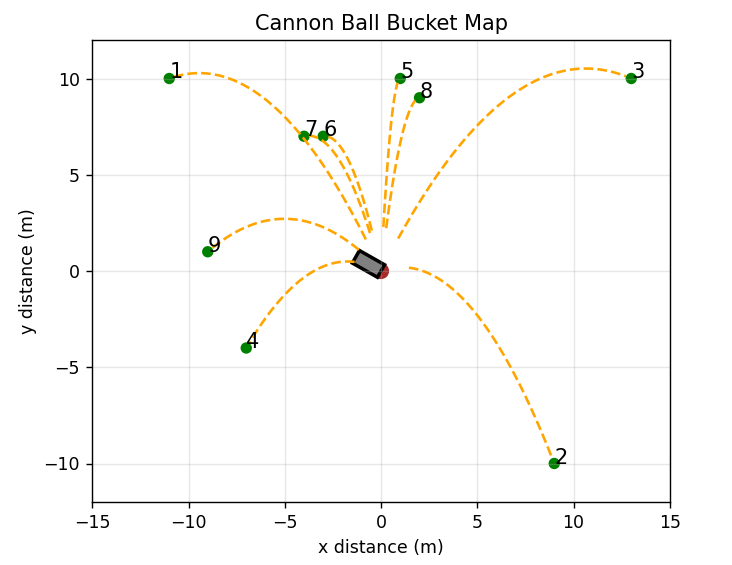
\includegraphics[width=0.5\linewidth]{images/Successful_Cannon_Sim.png}
    \caption{Example of a successfully ran Cannon Simulation}
\end{figure}

\noindent
\textbf{The Challenge} \\
\noindent
\textbf{Implement the \texttt{cannon\_code\_breaker} function to shoot buckets of known location in a 2D space in order given a code of non-repeating digits 1-9. Use the CannonSimulator class to test your code.} Try implementing both a brute force and an analytical solution, and poke around with how changing the simulations parameters impacts your solution. \\

\noindent
\textbf{Deliverable}\\
It is expected that you are able to present your code and speak on the design choices you made and explain how tweaking parameters would change the outcome or your implementation. Please bring your solution to your interview. 

\end{document}
